%----------------------------------------------------------------------------------------
%	PACKAGES AND DOCUMENT CONFIGURATIONS
%----------------------------------------------------------------------------------------

\documentclass[
	letterpaper, % Paper size, specify a4paper (A4) or letterpaper (US letter)
	10pt, % Default font size, specify 10pt, 11pt or 12pt
]{class}

\usepackage{caption}
\usepackage{soul}
\usepackage{subcaption}

\addbibresource{bibliography.bib} % Bibliography file (located in the same folder as the template)

%----------------------------------------------------------------------------------------
%	REPORT INFORMATION
%----------------------------------------------------------------------------------------

\title{Airline Departure\\Data Analysis and Regression} % Report title

\author{Lucchi Manuele \& Tricella Davide} % Author name(s), add additional authors like: '\& James \textsc{Smith}'

\date{\today} % Date of the report

%----------------------------------------------------------------------------------------

\begin{document}

\maketitle % Insert the title, author and date using the information specified above

\begin{center}
    \begin{tabular}{l r}
        Instructors: Professor \textsc{Cesa-Bianchi} \& Professor \textsc{Malchiodi}
    \end{tabular}
\end{center}

%----------------------------------------------------------------------------------------
%	DECLARATION
%----------------------------------------------------------------------------------------

\textit{We declare that this material,
    which we now submit for assessment, is entirely our own work and has not been
    taken from the work of others, save and to the extent that such work has been cited and
    acknowledged within the text of our work. We understand that plagiarism, collusion,
    and copying are grave and serious offences in the university and accept the penalties that
    would be imposed should I engage in plagiarism, collusion or copying. This assignment,
    or any part of it, has not been previously submitted by us or any other person for
    assessment on this or any other course of study.}

%----------------------------------------------------------------------------------------
%	ABSTRACT
%----------------------------------------------------------------------------------------

\begin{abstract}
    The purpose of this paper is to evaluate the usage of a Logistic Regression model on a airlines dataset to predict flight cancellation or diversion, in a scalable and time/space efficient implementation.
\end{abstract}

%----------------------------------------------------------------------------------------
%	TOC
%----------------------------------------------------------------------------------------

\tableofcontents

%----------------------------------------------------------------------------------------
%	DEFINITIONS
%----------------------------------------------------------------------------------------

\section{Definitions}\label{definitions} % Labels provide a point for referencing, in this case with \ref{definitions} to refer to this subsection number

\begin{description}
    \item[Dataset] The sample of data used to train the Model
    \item[Label] The expected outcome of the prediction
    \item[Model] The group of algorithms that tries to solve the problem
    \item[Overfitting] When the model is too sensible to changes compared to the dataset
    \item[Vanishing Gradient] When the gradient values becomes progressively smaller until they are insignificant for the process
\end{description}

%----------------------------------------------------------------------------------------
%	INTRODUCTION
%----------------------------------------------------------------------------------------

\section{Introduction}

The paper is splitted in a describing part, where the operations on the dataset and how the model is built are detailed, and an experimental part where a series of tests are performed and the results are stated.\\

Also, the document covers two different objectives, the classification of the dataset using the model to predict both the \textbf{canceled} and the \textbf{diverted} flights.\\
The two objectives are virtually the same, since the subset of the dataset used is identical and the model stays the same.\\

Both the cases represent real world problems that are still not completely solved, since there aren't algorithms that predicts these situations with accuracy yet, so a simple Logistic Regression model is probably not enough powerful to accomplish this tasks, but it's still worth analyzing its behavior in different circumstances.

%----------------------------------------------------------------------------------------
%	DATASET
%----------------------------------------------------------------------------------------

\section{Dataset}

The initial dataset, "Airline Delay and Cancellation Data" \cite{dataset} is made of 9 years of airlines flights data, composed by 10 files (one for each year from 2009 to 2018) with around 6 milions records each.
The files presents 28 columns, of which only the 9 more relevant were took\\

\begin{description}
    \item[FL\_DATE] The flight date.
    \item[OP\_CARRIER] The carrier code.
    \item[ORIGIN] The departure airport.
    \item[DEST] The destination airport.
    \item[CRS\_DEP\_TIME] The planned departure time.
    \item[CRS\_ARR\_TIME] The planned arrival time.
    \item[CANCELLED] If the flight has been canceled.
    \item[DIVERTED] If the flight has been diverted.
    \item[CRS\_ELAPSED\_TIME] The planned total time of the flight, taxi time included.
    \item[DISTANCE] The distance the flight has to cover.\\
\end{description}

The majority of columns have been excluded because contained information not available at departure time, like the ones regarding actual departure, flight and arrival time, which are at disposal only after the aircraft landed.
Other columns also contained informations which do not have any correlation with the objective of the experiments, like the flight number assigned by the carrier.\\

In the case the prediction is about the cancellation, the \texttt{DIVERTED} column will be ignored, while if the prediction is on if the flight would be diverted or not, the \texttt{CANCELLED} column will be ignored.\\

The carrier code is a two characters alphanumeric code, the origin and destination places are a three characters alphanumeric code.\\
Flight date, departure time and arrival time are dates, while the elapsed time and the distance are real numbers.\\
Cancelled and diverted are either 0 or 1.\\

500,000 records sampled with an uniform distributed were took from each year file to perform the preprocessing.

%----------------------------------------------------------------------------------------
%	PREPROCESSING
%----------------------------------------------------------------------------------------

\section{Preprocessing Techniques}

\subsection{Data processing}

Multiple preprocessing techniques were used.\\

Initially the rows without valid key values are removed, while the ones with invalid data the columns for which is possible to assign a default value are eventually corrected.\\

Then the data not already represented as real numbers has been converted; airports and carriers identifiers, that were alphanumeric codes, had a number assigned based on the code. Dates were splitted between the year and the rest, the former has been discarded, while the latter has been hashed.\\

\subsubsection{Hashing}

Particularly, to convert the identifiers, the checksum function \textbf{crc32} \cite{crc32} has been used, then the result has been put in END with the bytes representing the number -1, to ensure to get an unsigned integer. Finally, the value is normnalized dividing it for the max integer value.
This function has been choosen because is one of the fastest way to hash short strings, which is what is needed here, compared to other alghoritims like the SHA or MD5.\\

\subsubsection{Normalization}

To normalize dates, the day of the year has been extracted from every date, then divided by 365. A similar strategy has been used for the departure and arrival times, exctracting the minutes of the day and then dividing by 1140.\\

The distance has been normalized by dividing it for the maximum value found in the dataset, rounded by excess to 4970.\\

At this point, the dataset has been balanced in regard of the evaluated property, be it being canceled or diverted, so that there are an equal number of uniformly drawn positives and negatives.\\

The converted values were also limited between 0 and 1, to avoid exploding values during the training of the dataset.\\

Finally, the resulting dataset has been normalized by subtracting the \textbf{mean} and dividing by the \textbf{standard deviation}. This is called \textbf{Standard Score} \cite{normalization}.

$$ z = \frac{x - \mu}{\sigma} $$

\subsubsection{Balancing}

This was necessary since the diverted or cancelled flights are a really small percentage of the overall flights,
this in the first tests has been proved to be a problem, because the trained model always responded that no flight would have been cancelled or diverted, since it has been trained on a dataset with basically zero problematic flights.
To solve the problem an \textbf{Oversampling} has been applied, matching the number of normal flights and problematic flights.\\
Since less than 0.1\% of the dataset are positive cases (for both the tasks) after the oversampling, just 20000 of records could be used for the experiments, half with positive outcomes and half with negative ones.

\subsubsection{Splitting}
Lastly, the data was splitted between the \textbf{training set} (75\%) and the \textbf{test set} (25\%).\\

\subsection{Parallelization}

\subsubsection{PySpark}
Keeping in mind that the implementation has to be space and time efficient and \textbf{scale up to large datasets}, the preprocessing part has been carried out using the library PySpark.
PySpark is a wrapper for Python of the library Apache Spark \cite{spark}, originally written in Java.\\

The purpose of this library is the handling of \textbf{parallelized data processing}, particularly regarding the Distributed File System Hadoop, also created by the Apache Foundation.
The library handles automatically the work distribution on the available nodes that the system provide, it can be composed of a single machine with multiple cores or a cluster of machines, this improves significantly the \textbf{scalability} of the solution, which can be run on competely different system without code modification.\\

\subsubsection{Compatibility}

The usage of this library created some compatibility issues, because the data structures used by PySpark were not compatible with various parts of the preprocessing section, which had been written initially using the data science library Pandas \cite{pandas}.
To solve these problems, it wasn't possible to simply use a conversion and leave the parts written in Pandas as they were, because the computation would have run on a single machine, without parallelization, making the use of PySpark completely pointless.
The issue has been addressed using the \textbf{PySpark.SQL} functionality, which allow to execute queries on a distributed dataframe. For our purposes various UDF (User Defined Functions), have been created, which then have been applied to every column containing certain types of data.\\

\subsubsection{I/O}

The library PySpark is also able to handle the csv file reading and writing, so it has been used to save the preprocessed data to speed up multiple runs on the dataset. To carry out the writing of the various distributed dataframes, various files are created, then at the time of reading, the data is distributed to the various nodes. The data saved on the intermediate CSV is valid for both the tasks that are the goal of the paper.\\

\subsubsection{Integration}

The preprocessing part of the solution is therefore computed in a distributed manner, using the PySpark dataframe as main data structure to perform the various calculations on the columns of the dataset.
At the end of this section of the solution, the distributed dataframes are merged into one using the \texttt{collect} method. This operation can create memory problems if the dataset is extremely large, but the model training and computing can't be efficiently distributed
as easily as the preprocessing, so the main part of the solution will be computed using standard Python data structures.

%----------------------------------------------------------------------------------------
%	MODEL
%----------------------------------------------------------------------------------------

\section{Model}

The proposed model is a simple Logistic Regression \cite{logistic} algorithm that makes use of a few techniques to avoid overfitting (batching, L2 regularization) and uses the Gradient Descent as a solver.\\
The implementation uses \textbf{numpy} \cite{numpy} as its primary library of mathematical functions

\subsection{Parameters initialization}
Parameters such as Weights and Bias are initialized using a \textbf{uniform distribution} between 0 and 1, with the first one having the same length as the number of columns and the second being a scalar value.

\subsection{Algorithm}

\subsubsection{Estimate}
The estimate is computed as follows
$$ \hat{y} = \sigma(w^Tx + b) $$
where $\sigma$ is the Sigmoid function \cite{sigmoid} and it's defined as
$$ \sigma(z) = \frac{1}{1 + e^{-z}} \in [0,1] $$
and $w$ and $b$ are the model weights and bias and $x$ is the input.

The code implementation uses \texttt{np.exp} for the exponential calculation.

\subsubsection{Gradient}

$$ \nabla w = \frac{1}{m}x^T(\hat{y} - y) $$
$$ \nabla b = \frac{1}{m}\sum(\hat{y} - y) b $$

In the code implementation, \texttt{np.dot} and \texttt{np.mean} were used.

\subsubsection{Update}

Gradient Descent \cite{sgd} is a technique that allows to find maximus e minimum in a multi-variable function, like the model taken in consideration.\\
Once the gradients are calculated, the parameters (weights and bias in this case) will be updated with the gradient value properly mitigated with the \textbf{Learning Rate}

$$ w' = w - \mu \nabla w $$
$$ b' = b - \mu \nabla b $$

\subsubsection{Loss}
For the loss the \textbf{Binary Cross Entropy} \cite{binarycrossentropy} function, also called \textbf{Log Loss}, was used.
It is defined as
$$ loss(\hat{y}, y) = -\frac{1}{n}(y log(\hat{y}) + (1-y)log(1-\hat{y})) $$
This particular function is used since to perform the gradient descent it can be derived and conducted to the weights update formula to minimize it in the same way as it's done for the MSE \cite{mse} for the Linear Regression.\\

For the MSE and Linear Regression

$$ MSE(w) = \frac{1}{2} (\hat{y} - y)^2 = \frac{1}{2} (w^Tx - y)^2 $$
$$\frac{\partial J}{\partial w} = (w^T x - y)x $$
$$ w' = w - \mu (w^T x -y)x $$

For the Log Loss and Logistic Regression

$$ LogLoss(\hat{y}, y) = -y log \hat{y} - (1-y)log(1- \hat{y})$$
$$ \hat{y} = sigmoid(w^Tx) = \frac{1}{1 + e^{w^Tx}} $$
$$ \frac{\partial LogLoss}{\partial w} = (\hat{y} - y)x $$
$$ w' = w - \mu (\hat{y} - y)x $$
$$ w' = w - \mu (w^T x -y)x $$

\subsubsection{Batching}
There are multiple types of Gradient Descent.\\

\textbf{Stochastic Gradient Descent} updates the model after each sample and has a convergence rate that is non-linear $O(\frac{1}{k})$ where $k$ is a fixed step size.\\

\textbf{Batching Gradient Descent} updates the model once per iteration using the whole dataset at once. It has a better convergence rate.\\

\textbf{Mini Batch Gradient Descent} \cite{batching} uses small chunks of samples, so it's a middle solution between the previous ones, but adds a new hyperparameter to tune, the \textbf{Batch Size}.\\
Its convergence rate is
$$O(\frac{1}{\sqrt{bk}} + \frac{1}{k})$$

In this project the last one was choosen after a dedicated experiment.

\subsubsection{Regularization}
Regularization is a technique used to prevent the overfittings. A regularization term is added to the optimization problem (i.e. the gradient calculation) to avoid overfitting.
The used version is called \textbf{L2}, also known as \textbf{Ridge Regression} \cite{l2}. MIGLIORARE\\

The regularization factor for the loss is defined as
$$ L2 = \frac{\lambda}{2}||w||^2 $$
where $L2$ is calculated as
$$ \frac{\lambda}{2}||w||^2 = \frac{\lambda}2{\displaystyle\sum_{j=1}^m w_j^2} $$ \\

The loss then becomes
$$ loss(\hat{y}, y) = -\frac{1}{n}(y log(\hat{y}) + (1-y)log(1-\hat{y})) + \boldsymbol{\frac{\lambda}{2}||w||^2} $$

While the weights gradients formula becomes
$$ \nabla w = \frac{1}{m}x^T(\hat{y} - y) \boldsymbol{+ \lambda w} $$

\subsection{Differences with Sklearn implementation}

In the following chapters the presented model performances will be compared with the Sklearn implementation \cite{logisticsklearn}, that has quite some differences.\\
First, the sklearn version doesn't use the SGD solver, it uses \textbf{L-BFGS-B - Software for Large-scale Bound-constrained Optimization} \cite{lbfgsb} instead, by default.
% http://users.iems.northwestern.edu/~nocedal/lbfgsb.html
For this reason, the solver doesn't need any form of Learning Rate.\\
Also, with this implementation, the L2 Regularization is enabled by default as well.

% https://medium.com/@aditya97p/l1-and-l2-regularization-237438a9caa6
% https://github.com/mag3141592/LogisticRegression/blob/master/L2RegularizedLogisticRegression.py
% https://satishkumarmoparthi.medium.com/logistic-regression-with-l2-regularization-using-sgd-from-scratch-893692b48362
% https://towardsdatascience.com/batch-mini-batch-and-stochastic-gradient-descent-for-linear-regression-9fe4eefa637c

%----------------------------------------------------------------------------------------
%	EXPERIMENTS
%----------------------------------------------------------------------------------------

\section{Experiments}

As stated in the previous secontions, before starting the experiments the dataset is composed by about 20000 records, whose 15000 are for the training set and 5000 for the test set.\\
They are sampled from each file following a uniform distribution and they are equally positives and negatives outcomes.

\subsection{Preprocessing Performance}

The table below summarizes the time required by the \textbf{Colab enviroment} to complete various parts of the preprocessing section.
The numbers represents seconds of execution.

\begin{center}
    \begin{tabular}{ |c|c|c|c|c|c| }
        \hline
        Section                           & Pandas    & PySpark Single Node & PySpark Multiple Nodes \\
        \hline
        Data reading                      & 20.12526  & 0                   & 41.72719                      \\
        Null values removal               & 3.96165   & 0                   & 112.14040                      \\
        Names conversion                  & 114.67961 & 0                   & 117.07912                      \\
        Dates conversion                  & 51.46286  & 0                   & 109.54266                      \\
        Times conversion                  & 125.54429 & 0                   & 109.56157                      \\
        Distance conversion               & 69.56513  & 0                   & 110.38996                      \\
        Strings conversion (PySpark only) & -         & 0                   & 110.59919                      \\
        Column removal                    & 0.62132   & 0                   & 110.63221                      \\
        Balancing                         & 0.68836   & 0                   & 256.77912                      \\
        Splitting                         & 0.045422  & 0                   & 1145.30147                      \\
        Total                             & 366.01487 & 0                   & 2223,75289                      \\

        \hline
    \end{tabular}
    \captionof{table}{Performance comparison between Pandas preprocessing and distributed PySpark preprocessing}
\end{center}

Due to the limitations of the hardware used during the experiments, both locally and on Google Colab, we couldn't obtain significant improvements over preprocessing speed using PySpark, because of the lack of a high number of worker nodes.\\
DA RIFARE

\subsection{Canceled Flights}

The following sections represents the results about a series of experiments for the tuning of the hyperparameters of the model.

\subsubsection{Changing the Learning Rate}

The following experiment consists on the training and evaluation of the model with different values of the Learning Rate. The training is fixed at 100 iterations.

\begin{center}
    \begin{tabular}{ |c|c|c| }
        \hline
        LR     & Train Loss & Test Loss \\
        \hline
        0.1    & 0.68296    & 0.69123   \\
        0.01   & 1.12164    & 1.02453   \\
        0.001  & 1.27019    & 1.21357   \\
        0.0001 & 1.11576    & 1.30633   \\
        \hline
    \end{tabular}
    \captionof{table}{Training and Test Loss for different values of the Learning Rate}
\end{center}

As the results shows, an higher learning rate seems to perform better, therefore a learning rate of 1 has been tried showing similar results.\\
This is an unexpected behavior, since usually the gradient descent performs better with a lower learning rate. Given the complexity of the problem for a simple model like the Logistic Regression, another experiment has been made to choose the best Learning Rate.\\

Using the Mini-Batch technique for $\mu=0.001$ and $Batch Size = 20$ (whose experiment will be detailed in the section below) a difference with this test can be found.

\begin{figure}[!h]
    \centering
    \begin{subfigure}{0.49\textwidth}
        \centering
        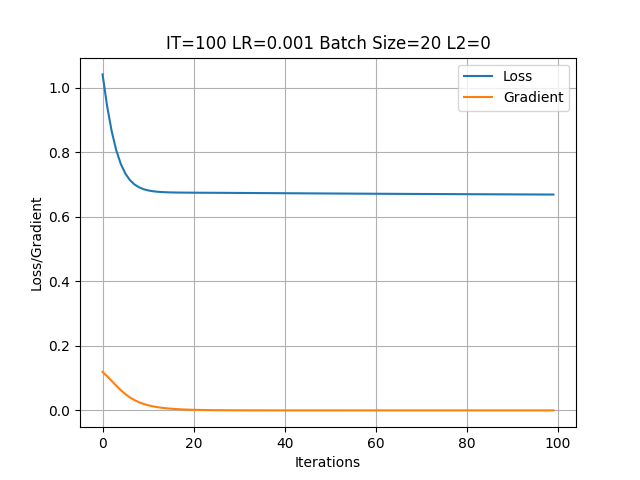
\includegraphics[width = \textwidth]{../images/graph_1.png}
        \caption{$\mu = 0.001$ and $Batch Size = 20$}
        \label{fig:left}
    \end{subfigure}
    \begin{subfigure}{0.49\textwidth}
        \centering
        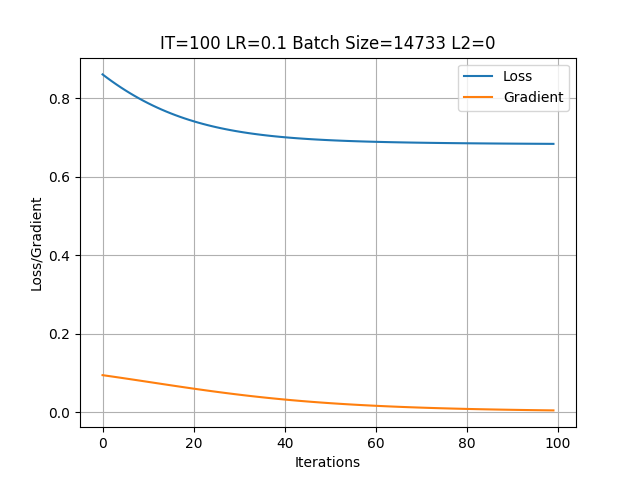
\includegraphics[width = \textwidth]{../images/graph_2.png}
        \caption{$\mu = 0.1 $ and $Batch Size = Max$}
        \label{fig:right}
    \end{subfigure}
    \label{fig:combined}
\end{figure}

As the charts shows, while both the hyperparameters configurations converge to the same (local) minimum, the one that uses mini batch and a lower learning rate convergence at a much faster speed.
In the following experiments, this configuration will be the one used.

\subsubsection{Implementing Mini-Batch}

As anticipated before, the mini-batch technique has been used. Being able to train the model with a fraction of the dataset at time resulted in a great reduction of the loss.

\begin{center}
    \begin{tabular}{ |c|c|c| }
        \hline
        Batch Size & Train Loss & Test Loss \\
        \hline
        1          & 0.37784    & 1.02391   \\
        20         & 0.60918    & 0.70032   \\
        1000       & 1.23453    & 0.92476   \\
        Max        & 1.02630    & 1.01142   \\
        \hline
    \end{tabular}
    \captionof{table}{Training and Test Loss for different size of batches}
\end{center}

In the first case, the model has been updated for each sample. This caused a degradation on performances and while the training loss is low, the test loss is three times higher, which lead to think the model is overfitted.\\

In the second case, the test loss is much lower and similar to the train loss, while on the last two cases it's just a worse result in general. Thus, for the next experiments, a \textbf{Batch Size of 20} has been chosen.

\subsubsection{Adding the L2 regularization}

As described before, to avoid overfitting, a regularization term has been added, in this case the L2.

\begin{center}
    \begin{tabular}{ |c|c|c| }
        \hline
        L2    & Train Loss & Test Loss \\
        \hline
        0     & 0.60740    & 0.70037   \\
        0.1   & 0.61829    & 0.69714   \\
        0.01  & 0.61010    & 0.69960   \\
        0.001 & 0.60819    & 0.70023   \\
        \hline
    \end{tabular}
    \captionof{table}{Training and Test Loss for a different value of the L2 term}
\end{center}

Since the model didn't appear to be overfitting from the start, the regularization doesn't show any significant benefit.\\
The following experiments used $\lambda = 0.1$

\subsubsection{More iterations}

\begin{center}
    \begin{tabular}{ |c|c|c| }
        \hline
        Iterations & Train Loss & Test Loss \\
        \hline
        100        & 0.60978    & 0.69974   \\
        200        & 0.60978    & 0.69969   \\
        1000       & 0.60962    & 0.69971   \\
        \hline
    \end{tabular}
    \captionof{table}{Training and Test Loss for different number of iterations}
\end{center}

Increasing the number of iterations didn't lead to any noticeable improvement.

\subsubsection{ROC Curve}

The apparently better performing configuration of the hyperparameters has the following \textbf{ROC curve}

\begin{center}
    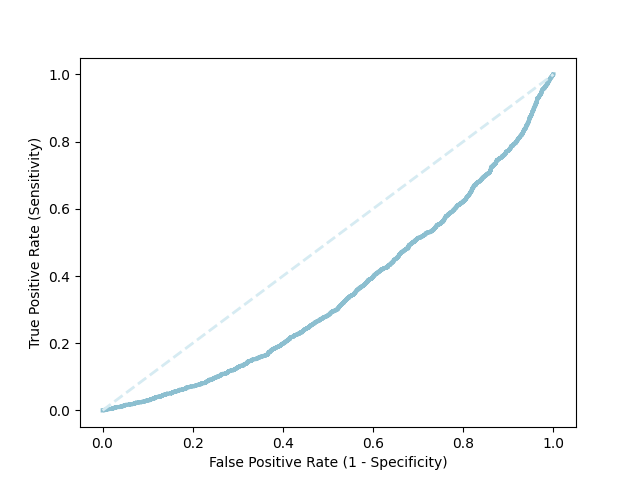
\includegraphics[width=10cm]{../images/roc_1.png}
    %\captionof{$\mu = 0.001$ and $Batch Size = 20$}
    %\label{roc1}
\end{center}

It has a decent ability to predict, but as an inverse predictor, suggesting that mini batch feature

A notable case is the experiment with the same learning rate but without the Mini Batch feature.

\begin{center}
    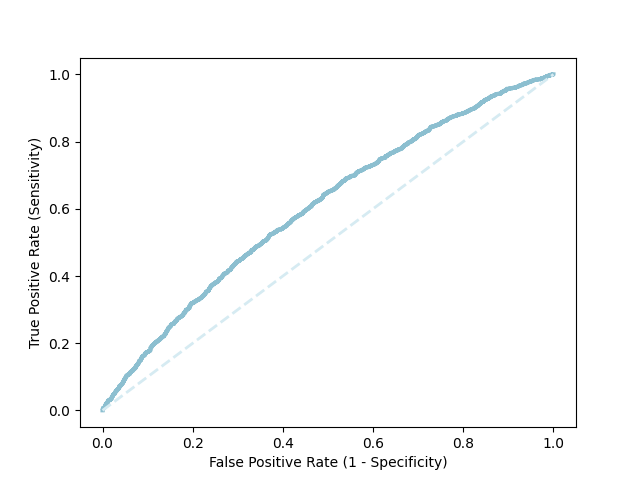
\includegraphics[width=10cm]{../images/roc_2.png}
    %\captionof{$\mu = 0.001$ and $Batch Size = Max$}
    %\label{roc2}
\end{center}

It has a similar curve to the previous case, but this time it's not predicting the inverse. This is interesting since the loss of this configuration is really high loss and it suffers of vanishing gradient as can be seen from the following chart

\begin{center}
    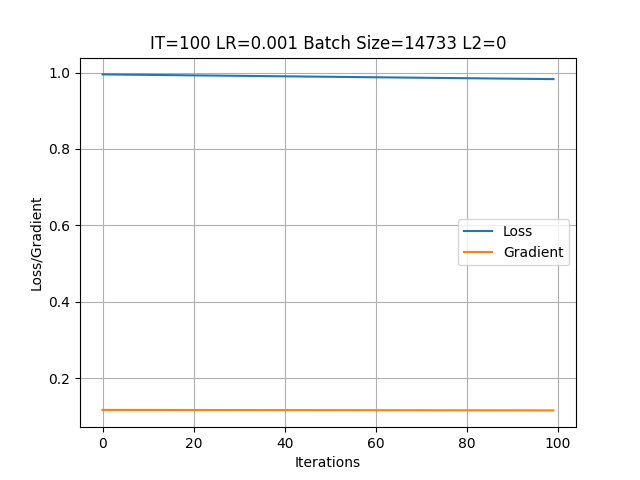
\includegraphics[width=10cm]{../images/graph_3.png}
    %\captionof{$\mu = 0.001$ and $Batch Size = Max$}
    %\label{graph3}
\end{center}

It's safe to say that this model is not really reliable, and just underfitted.

\subsubsection{Comparison with Sklearn}

To conclude the experiments, the instance with the best hyperparameters from the previous experiments has been compared with the Sklearn implementation.\\

The Sklearn one uses the same number of iterations and uses L2 regularization, but doesn't use the SGD (and thus the Learning Rate) or the batching.
Instead it uses \textbf{L-BFGS-B} \cite{lbfgsb}, a solver for Large-scale Bound-constrained Optimization.

\begin{center}
    \begin{tabular}{ |c|c|c|c|c|c|c| }
        \hline
        Model   & Iterations & LR    & Batch Size & L2      & Train Loss & Test Loss \\
        \hline
        Custom  & 100        & 0.001 & 20         & 0.1     & 0.60978    & 0.69974   \\
        Sklearn & 100        & N/A   & N/A        & Unknown & N/A        & 0.66953   \\
        \hline
    \end{tabular}
    \captionof{table}{Training and Test Loss comparison with Sklearn with the best hyperparameters values for both}
\end{center}

The results are very close, with the Sklearn implementation being slightly better.

\subsection{Diverted Flights}

As stated before, the two problems (canceled and diverted flights) are virtually the same problem. They are both a binary classification and both uses the same columns, since they are influenced by the same factors and all are known until before the takeoff.\\

For this reason, the results obtained are equivalent, so they will just be reported in the following sections, with the comments for the previous section being valid for this one.

\subsubsection{Changing the Learning Rate}

\begin{center}
    \begin{tabular}{ |c|c|c| }
        \hline
        LR     & Train Loss & Test Loss \\
        \hline
        0.1    & 0.67999    & 0.69171   \\
        0.01   & 0.90016    & 0.91724   \\
        0.001  & 0.94824    & 1.16871   \\
        0.0001 & 1.03176    & 1.30609   \\
        \hline
    \end{tabular}
    \captionof{table}{Training and Test Loss for different values of the Learning Rate}
\end{center}

\subsubsection{Implementing Mini-Batch}

\begin{center}
    \begin{tabular}{ |c|c|c| }
        \hline
        Batch Size & Train Loss & Test Loss \\
        \hline
        1          & 0.17018    & 0.99730   \\
        20         & 0.61886    & 0.69662   \\
        1000       & 1.24722    & 1.13225   \\
        Max        & 0.93345    & 1.03499   \\
        \hline
    \end{tabular}
    \captionof{table}{Training and Test Loss for different size of batches}
\end{center}

\subsubsection{Adding the L2 regularization}

\begin{center}
    \begin{tabular}{ |c|c|c| }
        \hline
        L2    & Train Loss & Test Loss \\
        \hline
        0     & 0.61563    & 0.69760   \\
        0.1   & 0.62842    & 0.69513   \\
        0.01  & 0.61832    & 0.69720   \\
        0.001 & 0.61989    & 0.69576   \\
        \hline
    \end{tabular}
    \captionof{table}{Training and Test Loss for a different value of the L2 term}
\end{center}

\subsubsection{More iterations}

\begin{center}
    \begin{tabular}{ |c|c|c| }
        \hline
        Iterations & Train Loss & Test Loss \\
        \hline
        100        & 0.62105    & 0.69645   \\
        200        & 0.61847    & 0.69721   \\
        1000       & 0.61822    & 0.69749   \\
        \hline
    \end{tabular}
    \captionof{table}{Training and Test Loss for different number of iterations}
\end{center}

\subsubsection{Comparison with Sklearn}

\begin{center}
    \begin{tabular}{ |c|c|c|c|c|c|c| }
        \hline
        Model   & Iterations & LR    & Batch Size & L2      & Train Loss & Test Loss \\
        \hline
        Custom  & 100        & 0.001 & 20         & 0.1     & 0.62105    & 0.69645   \\
        Sklearn & 100        & N/A   & N/A        & Unknown & N/A        & 0.67672   \\
        \hline
    \end{tabular}
    \captionof{table}{Training and Test Loss comparison with Sklearn with the best hyperparameters values for both}
\end{center}


%----------------------------------------------------------------------------------------
%	RESULTS AND CONCLUSIONS
%----------------------------------------------------------------------------------------

\section{Results and Conclusions}

The reason of this experiments was to reproduce a complete flow to create and train a Logistic Regression model to classify flights data.\\
The dataset preprocessing has been successfully parallelized using PySpark, but the lack of a proper distributed system to test on lead to worse performances compared to the pandas implementation.\\
Instead, the model built using SGD, L2 Regularization, Normalization and Batching (properly tuned) resulted in an accuracy similar to the state-of-art Sklearn implementation.\\
Both of the models probably converged on a local minimum, that would explain the high loss, and this could be explained by the Logistic Regression being a weak model for a real world complex problem like the one taken in consideration.

%----------------------------------------------------------------------------------------
%	BIBLIOGRAPHY
%----------------------------------------------------------------------------------------

\printbibliography % Output the bibliography

% Logistic Regression
% Spark/PySpark
% Kaggle Dataset
% Mini Batch
% L2 Regularization
% Normalization
% SGD
% Il solver di Sklearn
% sklearn, numpy, pandas
% binary cross entropy
% sigmoid

%----------------------------------------------------------------------------------------

\end{document}

% todo

% DEFINIZIONI
% ESPERIMENTI PREPROCESSING
% Performances del modello
% Add Bold words
% README